\subsection{Hierholzer}

\begin{itemize}
\item Man will einen Weg finden, der alle Kanten durchläuft
\end{itemize}

\begin{figure}[h]
\centering
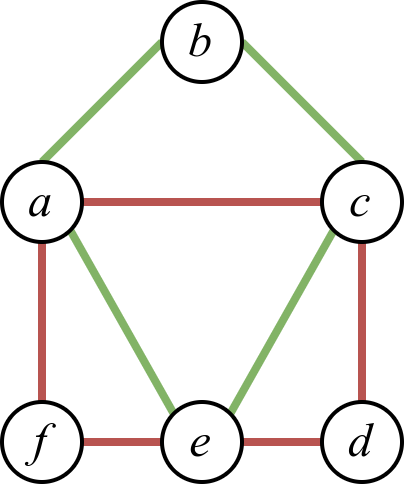
\includegraphics[width=0.2\textwidth]{graphics/hierholzer.png}
\end{figure}

\begin{itemize}
\item $R_1 = {\color{red}acdefa}$
\item $R_2 = {\color{Green}eabce}$
\item $R_1 + R_2 = {\color{red}acde\color{Green}abce\color{red}fa}$
\end{itemize}

\subsection{Prim}

\begin{itemize}
\item \textbf{Ziel:} Erstellung eines minimalen Spannbaum, von einem gewichteten ungerichteten Graphen.
\item Die Kantengewichte sind im vorhinein nicht bekannt
\item Es wird immer die Kante mit dem kleinsten Gewicht (welches aktuell bekannt ist) benutzt
\end{itemize}

\begin{figure}[h]
\centering
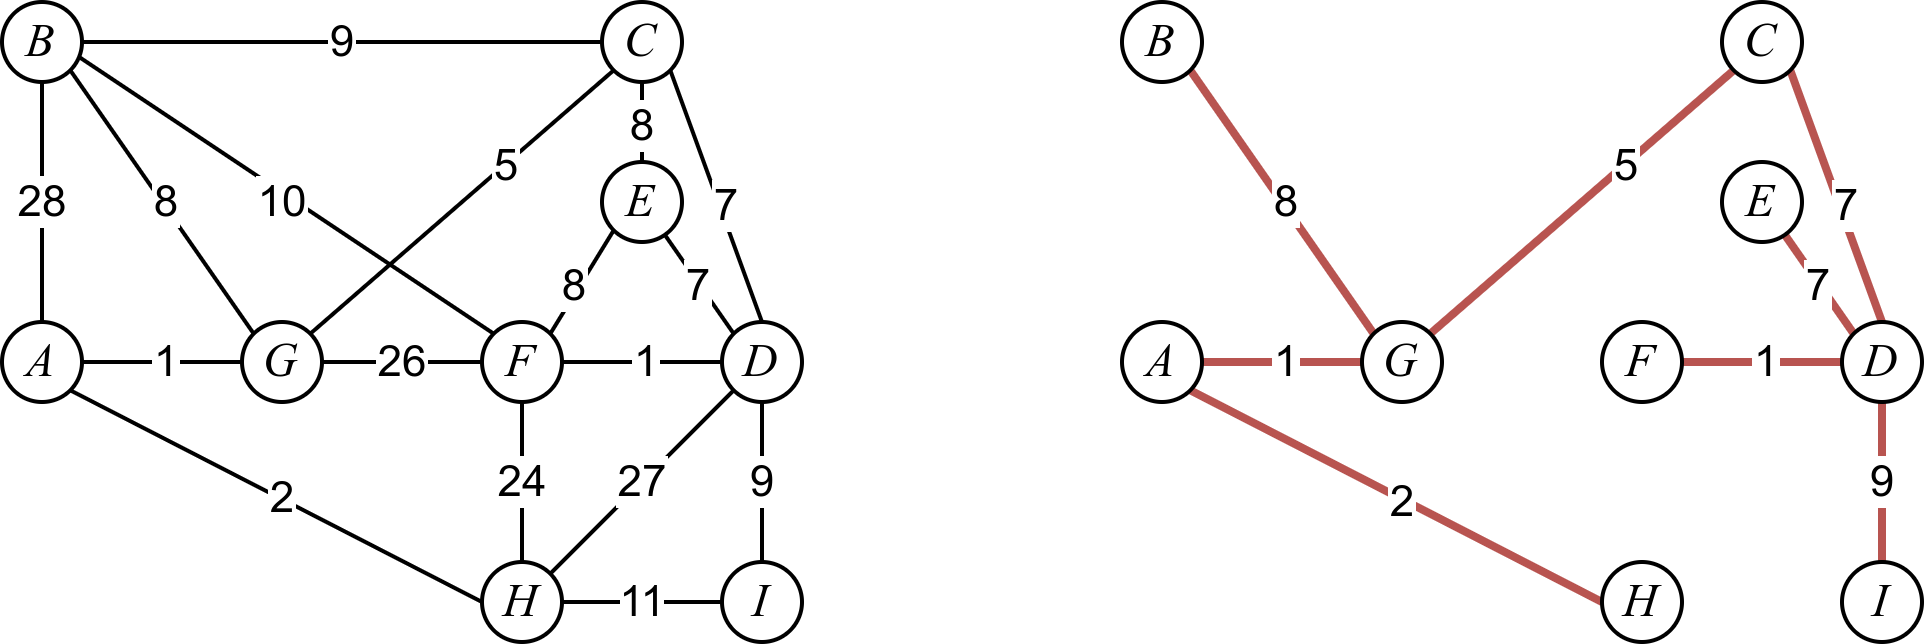
\includegraphics[width=0.7\textwidth]{graphics/prim_kruskal.png}
\end{figure}

\begin{itemize}
\item Start: ${A,G}$
\item Füge hinzu: ${A,H}$
\item Füge hinzu: ${G,C}$
\item Füge hinzu: ${C,D}$
\item Füge hinzu: ${D,F}$
\item Füge hinzu: ${D,E}$
\item Füge hinzu: ${B,G}$
\item Füge hinzu: ${D,I}$
\end{itemize}

\newpage

\subsection{Kruskal}

\begin{itemize}
\item \textbf{Ziel:} Erstellung eines minimalen Spannbaum, von einem gewichteten ungerichteten Graphen.
\item Alle Kantengewichte sind im vorhinein bekannt
\end{itemize}

\begin{figure}[h]
\centering
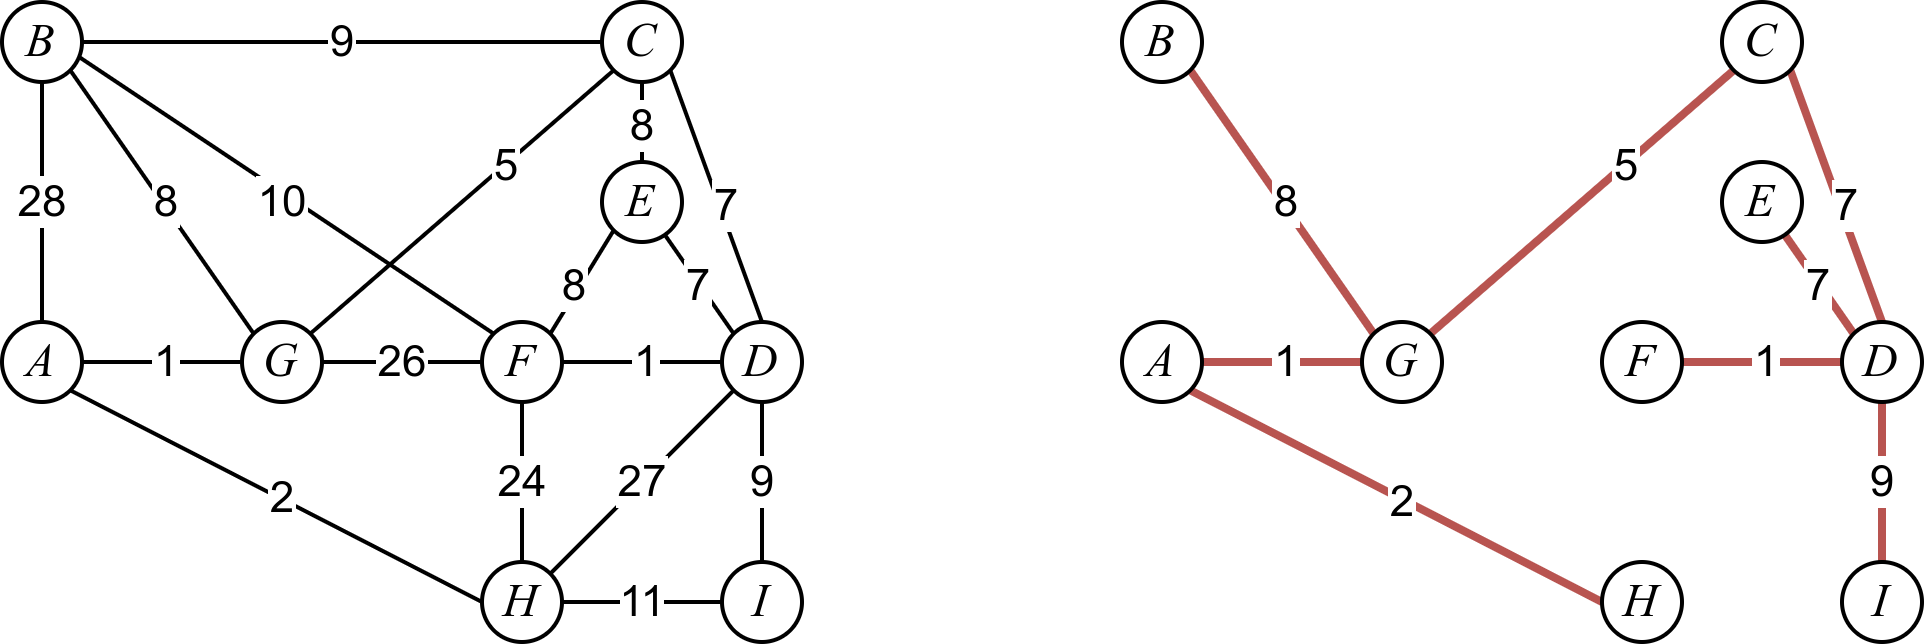
\includegraphics[width=0.7\textwidth]{graphics/prim_kruskal.png}
\end{figure}

\begin{itemize}
\item Start: ${A,G}$
\item Füge hinzu: ${F,D}$
\item Füge hinzu: ${A,H}$
\item Füge hinzu: ${G,C}$
\item Füge hinzu: ${F,D}$
\item Füge hinzu: ${C,D}$
\item Füge hinzu: ${D,E}$
\item Füge hinzu: ${G,B}$
\item Füge hinzu: ${D,I}$
\end{itemize}